\chapter{Appendix: Evaluating polaris\textasciitilde{}}
\markboth{}{Appendix: Evaluating polaris\textasciitilde{}}

\noindent \textbf{Project Blog:}        \url{https://www.sambilbow.com/projects/polaris}

\noindent \textbf{Project Code:}        \url{https://www.github.com/sambilbow/polaris}

\noindent \textbf{Project Guide:}       \url{https://www.github.com/sambilbow/polaris/wiki}

\noindent \textbf{Project Publication } \url{https://doi.org/10.21428/92fbeb44.8abb9ce6}

\section{Blog Contents}
\section{Code Repository}
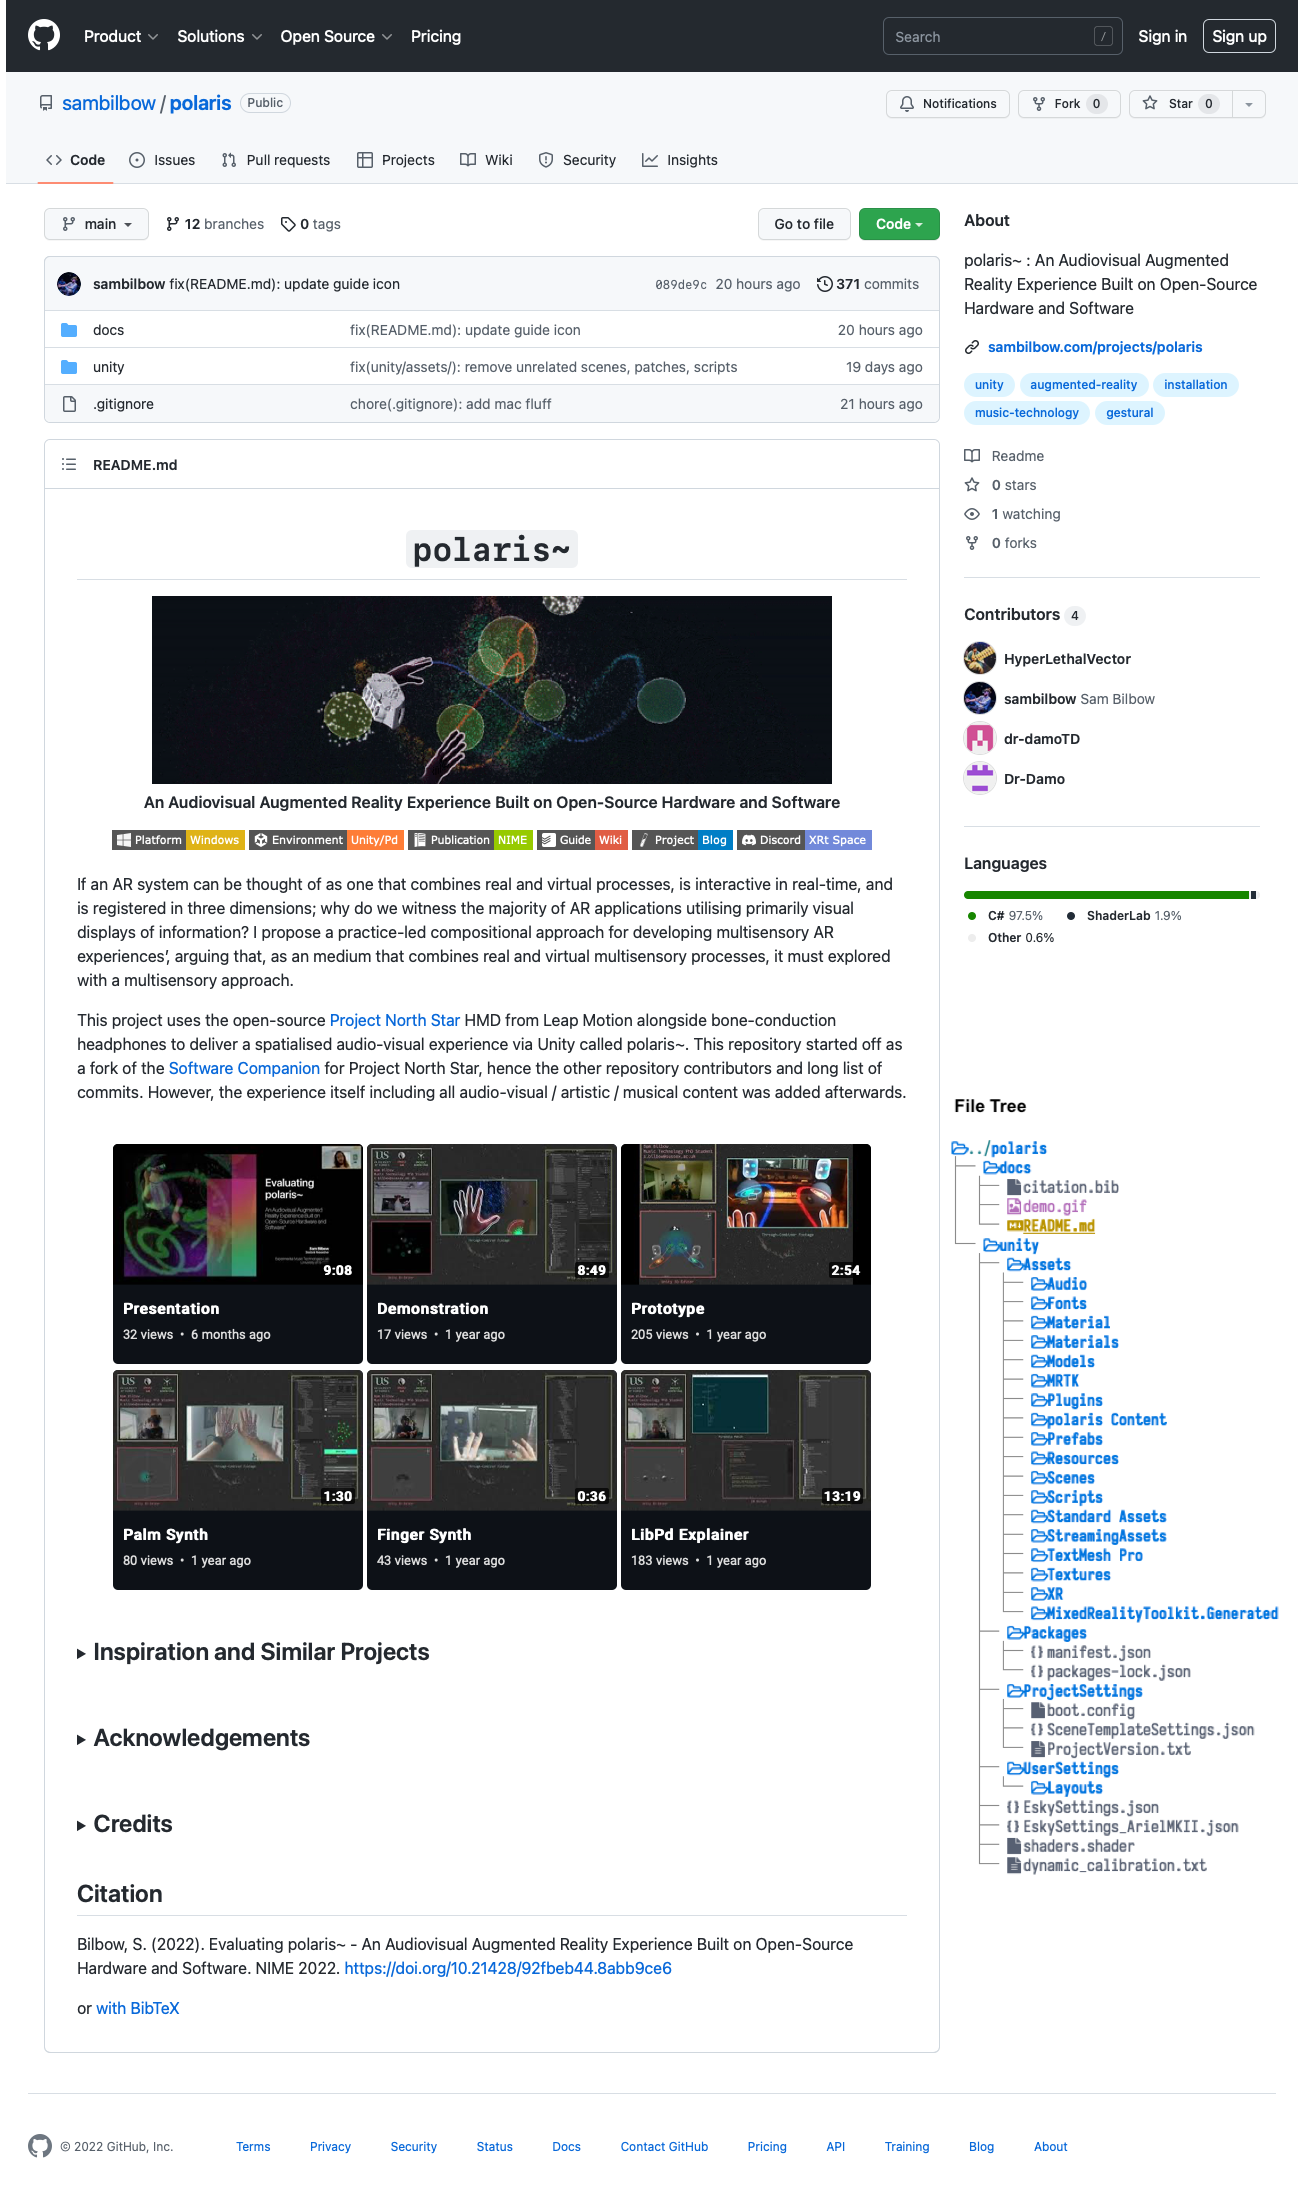
\includegraphics[width=\textwidth,height=\textheight,keepaspectratio]{10-appendix-b/polaris-code-file.png}
\section{Project Guide}
% --------------------------------------------------------------------------- %
\section{NIME'22 Ethics Statement}\label{sec: polaris-ethics}
The study followed University of Sussex ethics guidelines approved by the Social Sciences \& Arts Cross-Schools Research Ethics Committee with the reference code: ER/SMB44/3.

\subsection{Socio-economic Fairness}\label{sec: polaris-ethics-}
At all stages of this research, I have sought to minimise the outlay required to invest in technology needed to implement \textit{polaris\textasciitilde{}}. This has meant opting for FLOSS (free / libre open-source software) where possible: The software companion to the North Star, Project Esky \footnote{`Esky' is a colloquial term for an ice-cooler in Australia, etymologically deriving from the word ‘Eskimo’. I acknowledge the use of this term as being pejorative towards the indigenous populations of the Greenlandic and Canadian Inuit, Alaskan Iñupiat, and Yupik peoples; fully recognise their human and land rights, and have made the effort to redact the word within the main body of this article.}, PureData, and OBS. Ideally the 3D-engine used would also be FLOSS, i.e. Godot, but due to time constraints I have opted for Unity which I am already experienced with, and which has great documentation and free learning materials.

Though the Project North Star headset is OSH (open-source hardware), I have not had time to develop DIY and OSH audio solution yet, but any bluetooth bone-conduction headphones are compatible.

Unfortunately, the \textit{polaris\textasciitilde{}} experience (and as such, its framework) is not compatible with macOS and Linux, although it will be once Ultraleap provide their V5 drivers for hand-tracking on those operating systems.

It is worth noting that, as with most smaller suppliers of technology, the current global chip shortage has made getting hold of some components quite difficult at times, and recently the developers of the display driver board had to take the time to redesign it to get around this; the headset was not available to buy new for several months during this period. I suppose that this points to an issue: \textit{``accessibility"} doesn’t always correlate with \textit{``availability"}, especially when trying to circumvent expensive consumer technologies.

Since beginning these studies, Intel has discontinued their T261/T265 range of products, meaning that anyone looking to build the headset today would have difficulty including movement tracking, a fairly essential component of effective AR experiences. I am fully aware of the roadblock this puts in the way of \textit{polaris\textasciitilde{}} currently being reproducible as per its framework, but thankfully efforts are underway by developers in the community to solve this issue by migrating to Luxonis’ modular and open-source range of tracking cameras; leaving the proprietary and closed-source hardware and software of Intel behind. If anything, their announcement has served as a reminder of the importance of FOSS/H components in community-led projects.

\subsubsection{A note on the environment}\label{sec: polaris-ethics-environment}
While it is certainly difficult to mitigate the environmental impact entirely from projects that rely on technology, I have opted for compostable PLA material for the construction of the headset used in the study to reduce e-waste in the event of breakage or updates to the hardware design.

\subsection{Study Participants}\label{sec: polaris-ethics-participants}
\subsubsection{Accessibility}\label{sec: polaris-ethics-accessibility}
In anticipating the possibility of a diverse set of accessibility needs, I provided stepped and step-free access instructions to get to the lab, maintained clearly formatted correspondence with participants via e-mail, and observed the university’s COVID-19 policy during the study. Participants wearing glasses were able to use the headset with or without their glasses, and the volume of the AR scene was kept at a tolerable level, with the option given to participants to increase or decrease it.

\subsubsection{Inclusion}\label{sec: polaris-ethics-inclusion}
Participants were recruited via internal University undergraduate and postgraduate mailing lists and were selected to ensure a diverse cohort of individuals from differing ethnicities, genders, and ages.

\subsubsection{Remuneration}\label{sec: polaris-ethics-renumeration}
Study participants were compensated £15 each for the 45 minutes - 1 hour in which they took part in the study.

\subsubsection{Consent}\label{sec: polaris-ethics-consent}
All participants provided written consent to take part in the questionnaire, experience, and interview; and also to being video and audio recorded during this time. They could at any time choose not to participate further, without being penalised or disadvantaged in any way. Their involvement in the study did not in any way impact their marks, assessments, or future studies. After analysis, their transcribed contributions were approved, and they had the opportunity to remove any anonymous, but still sensitive information.

\subsubsection{Data and privacy}\label{sec: polaris-ethics-data}
Data from the studies: video and audio recordings, transcriptions, and analysis files are secured on a separate hard drive and are password protected. All quotes and data have been anonymised in accordance with data protection legislation.


% \section{polaris\textasciitilde{} Study Documents}

\includepdf[pages=1,pagecommand={\section{polaris\textasciitilde{} Study Documents} \subsection{Ethics Approval}}, scale=0.71, frame, offset=10mm 0]{figures/10-appendix-b/polaris-study-documents/ethics.pdf}

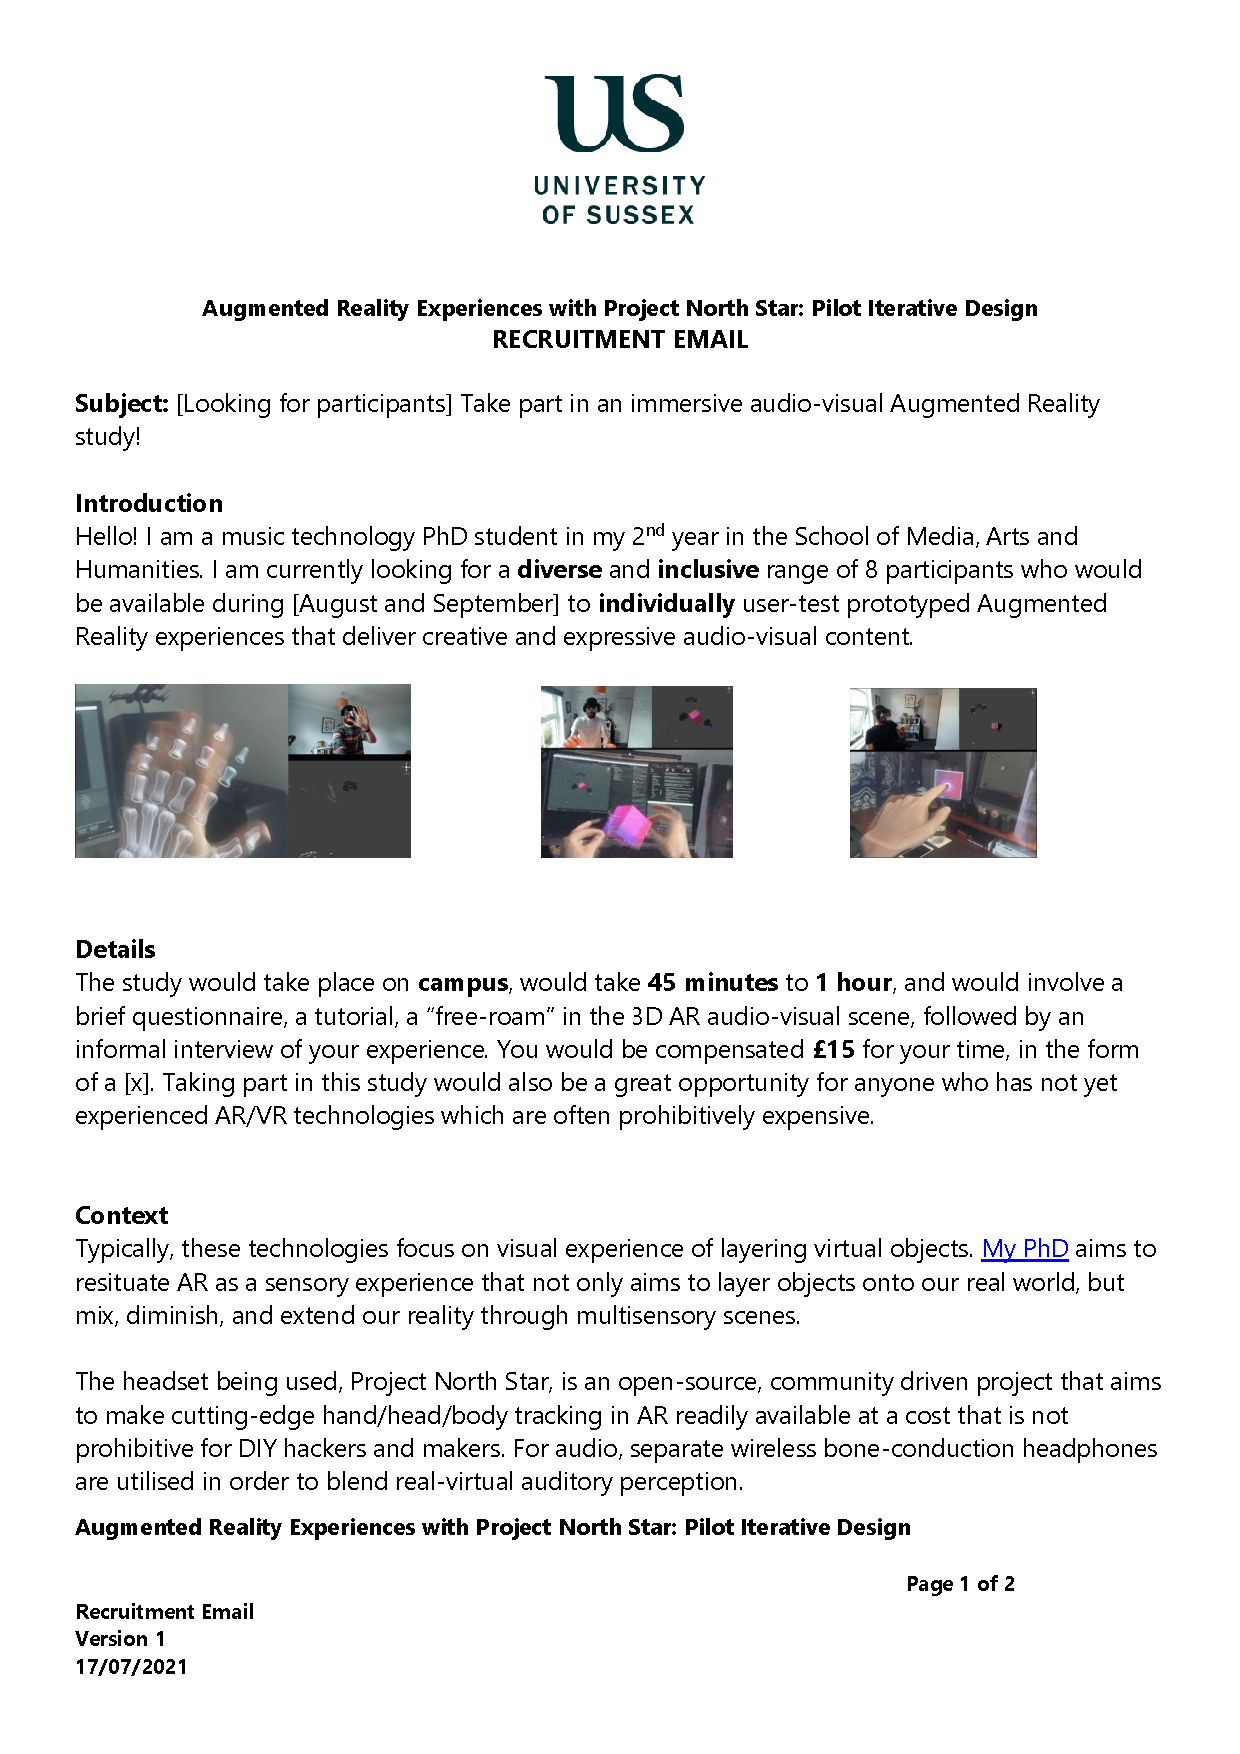
\includepdf[pages=1,pagecommand={\subsection{Recruitment}}, scale=0.71, frame, offset=10mm 0]{figures/10-appendix-b/polaris-study-documents/recruitment.pdf}
\includepdf[pages=2-,pagecommand={}, scale=0.71, frame, offset=10mm 0]{figures/10-appendix-b/polaris-study-documents/recruitment.pdf}


\includepdf[pages=1,pagecommand={\subsection{Information Sheet}}, scale=0.71, frame, offset=10mm 0]{figures/10-appendix-b/polaris-study-documents/information-sheet.pdf}

\includepdf[pages=2-,pagecommand={}, scale=0.71, frame, offset=10mm 0]{figures/10-appendix-b/polaris-study-documents/information-sheet.pdf}


\includepdf[pages=1,pagecommand={\subsection{Consent Form}}, scale=0.71, frame, offset=10mm 0]{figures/10-appendix-b/polaris-study-documents/consent-form.pdf}

\includepdf[pages=2-,pagecommand={}, scale=0.71, frame, offset=10mm 0]{figures/10-appendix-b/polaris-study-documents/consent-form.pdf}

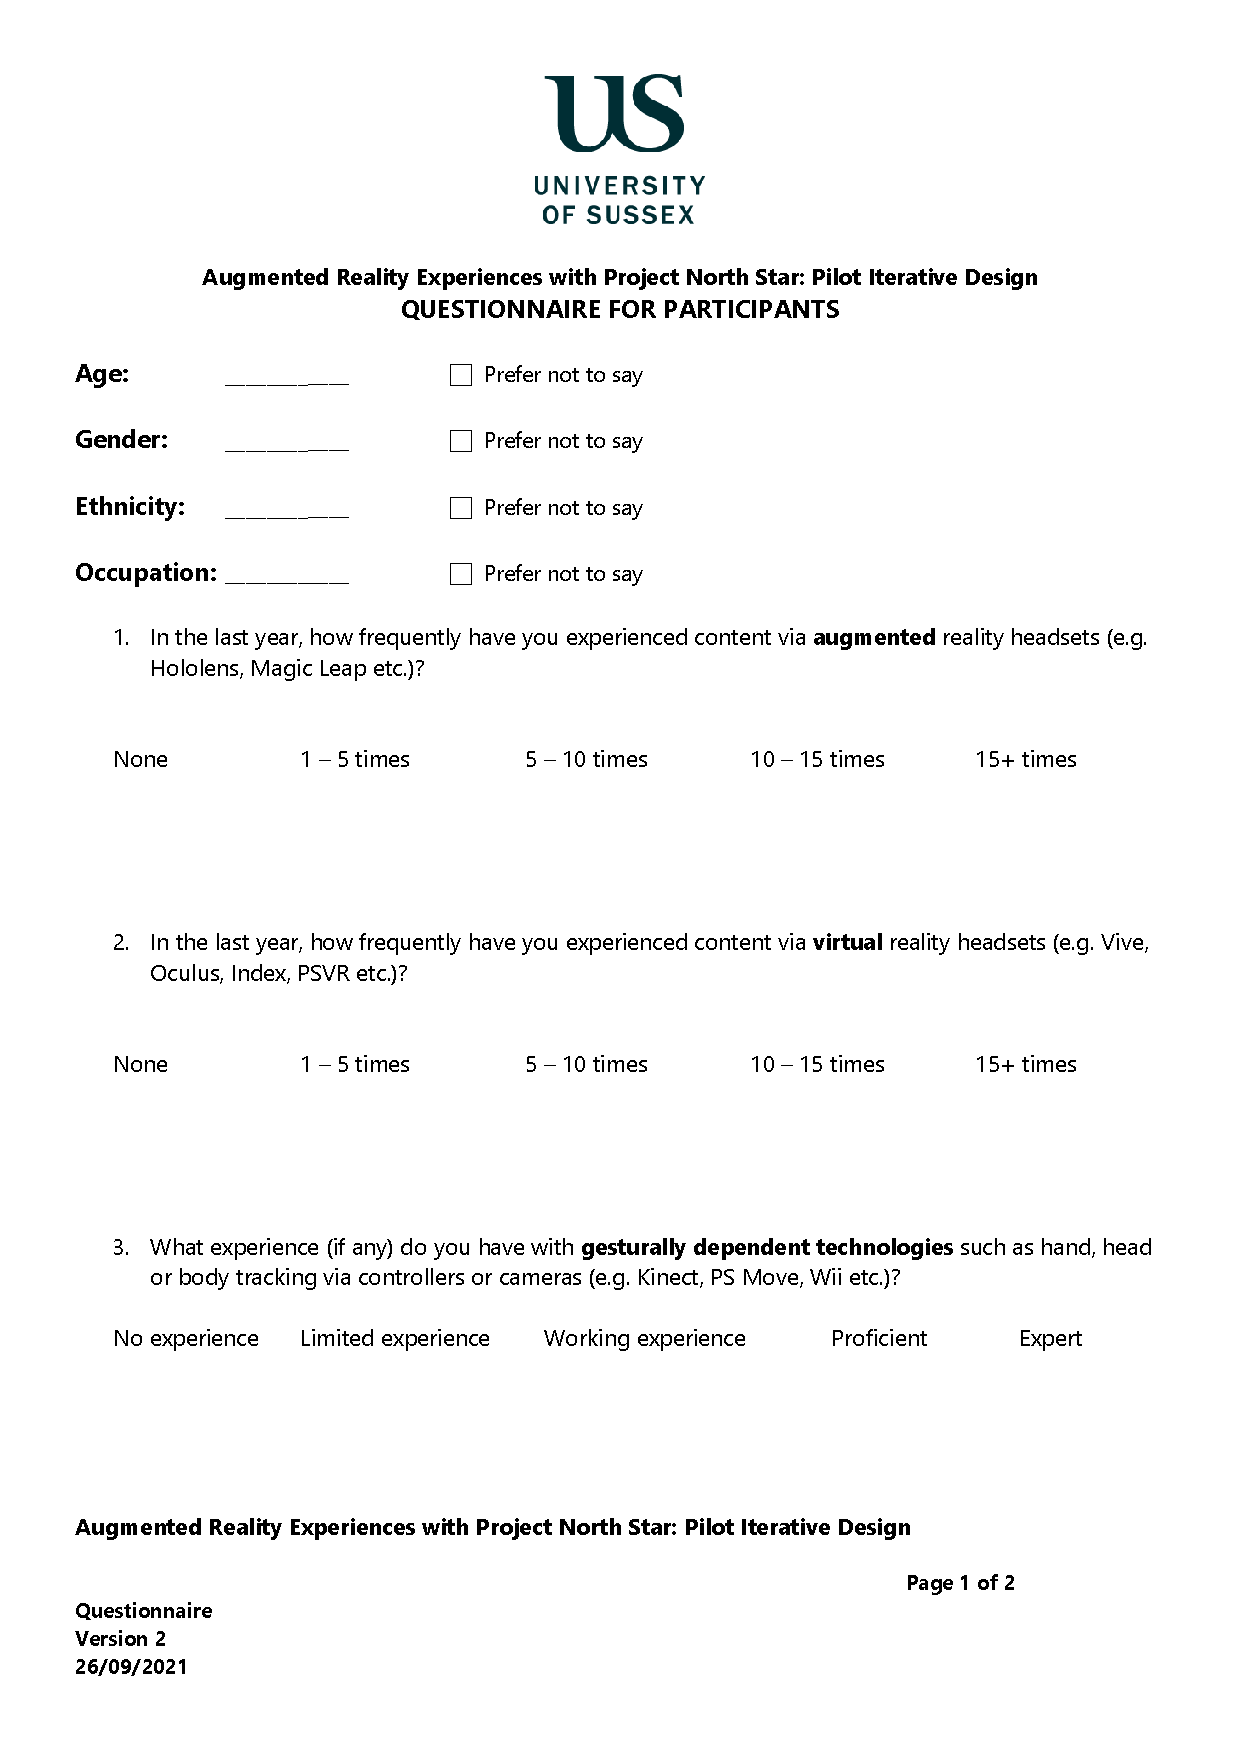
\includepdf[pages=1,pagecommand={\subsection{Questionnaire}}, scale=0.71, frame, offset=10mm 0]{figures/10-appendix-b/polaris-study-documents/questionnaire.pdf}
\includepdf[pages=2-,pagecommand={}, scale=0.71, frame, offset=10mm 0]{figures/10-appendix-b/polaris-study-documents/questionnaire.pdf}


\includepdf[pages=1-,pagecommand={\subsection{Tutorial}}, scale=0.71,nup=2x4,delta=2mm 2mm, frame, offset=10mm 0]{figures/10-appendix-b/polaris-study-documents/tutorial.pdf}

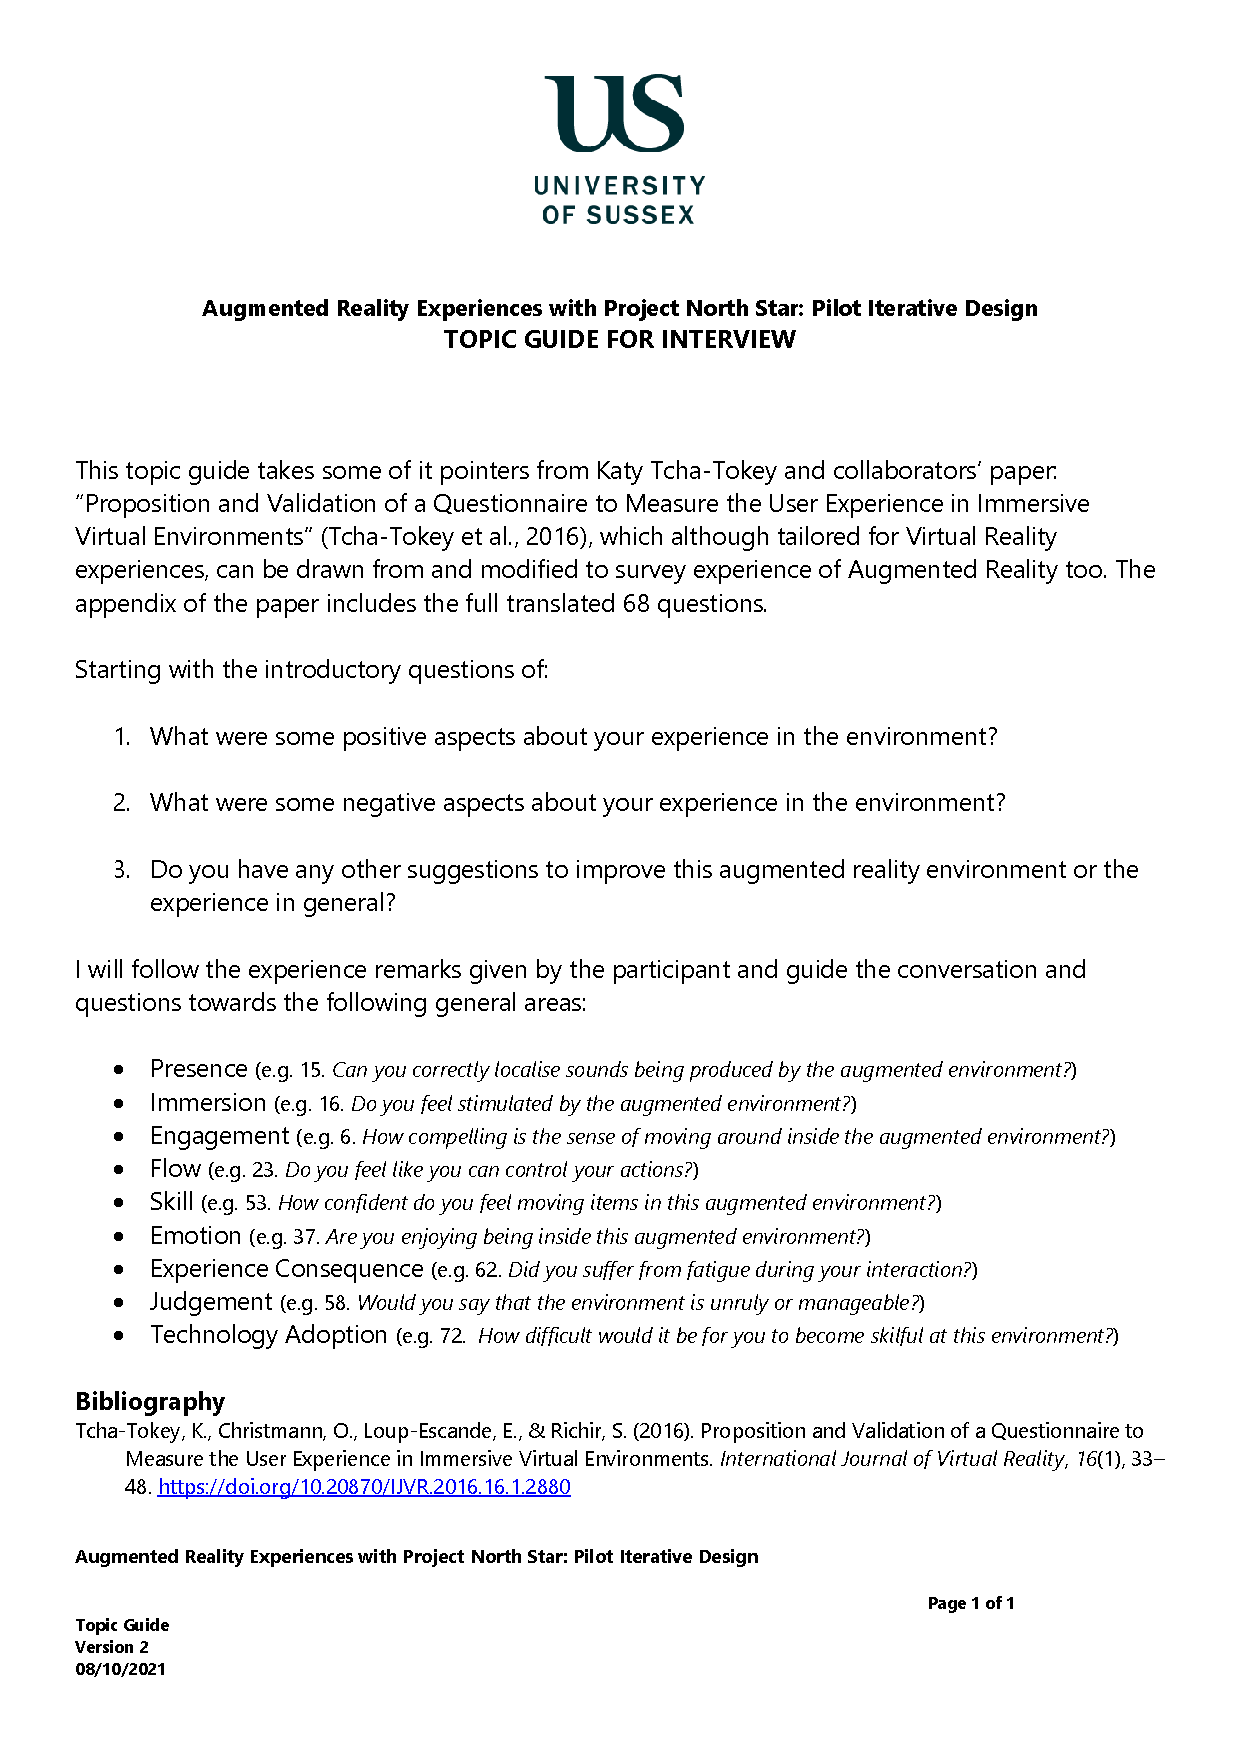
\includepdf[pages=1,pagecommand={\subsection{Interview Topic Guide}}, scale=0.71, frame, offset=10mm 0]{figures/10-appendix-b/polaris-study-documents/interview-topic-guide.pdf}
\includepdf[pages=2-,pagecommand={}, scale=0.71, frame, offset=10mm 0]{figures/10-appendix-b/polaris-study-documents/interview-topic-guide.pdf}

% \section{Transcriptions}
% \subsection{Participant 01}
% \subsubsection{Experience}
% \lstinputlisting{figures/10-appendix-b/polaris-study-documents/transcriptions/p01-experience.txt}
% \subsubsection{Interview}
% \lstinputlisting{figures/10-appendix-b/polaris-study-documents/transcriptions/p01-interview.txt}

% \subsection{Participant 02}
% \subsubsection{Experience}
% \lstinputlisting{figures/10-appendix-b/polaris-study-documents/transcriptions/p02-experience.txt}
% \subsubsection{Interview}
% \lstinputlisting{figures/10-appendix-b/polaris-study-documents/transcriptions/p02-interview.txt}

% \subsection{Participant 03}
% \subsubsection{Experience}
% \lstinputlisting{figures/10-appendix-b/polaris-study-documents/transcriptions/p03-experience.txt}
% \subsubsection{Interview}
% \lstinputlisting{figures/10-appendix-b/polaris-study-documents/transcriptions/p03-interview.txt}

% \subsection{Participant 04}
% \subsubsection{Experience}
% \lstinputlisting{figures/10-appendix-b/polaris-study-documents/transcriptions/p04-experience.txt}
% \subsubsection{Interview}
% \lstinputlisting{figures/10-appendix-b/polaris-study-documents/transcriptions/p04-interview.txt}

% \subsection{Participant 05}
% \subsubsection{Experience}
% \lstinputlisting{figures/10-appendix-b/polaris-study-documents/transcriptions/p05-experience.txt}
% \subsubsection{Interview}
% \lstinputlisting{figures/10-appendix-b/polaris-study-documents/transcriptions/p05-interview.txt}

% \subsection{Participant 06}
% \subsubsection{Experience}
% \lstinputlisting{figures/10-appendix-b/polaris-study-documents/transcriptions/p06-experience.txt}
% \subsubsection{Interview}
% \lstinputlisting{figures/10-appendix-b/polaris-study-documents/transcriptions/p06-interview.txt}

% \subsection{Participant 07}
% \subsubsection{Experience}
% \lstinputlisting{figures/10-appendix-b/polaris-study-documents/transcriptions/p07-experience.txt}
% \subsubsection{Interview}
% \lstinputlisting{figures/10-appendix-b/polaris-study-documents/transcriptions/p07-interview.txt}

% \subsection{Participant 08}
% \subsubsection{Experience}
% \lstinputlisting{figures/10-appendix-b/polaris-study-documents/transcriptions/p08-experience.txt}
% \subsubsection{Interview}
% \lstinputlisting{figures/10-appendix-b/polaris-study-documents/transcriptions/p08-interview.txt}

% \subsection{Participant 09}
% \subsubsection{Experience}
% \lstinputlisting{figures/10-appendix-b/polaris-study-documents/transcriptions/p09-experience.txt}
% \subsubsection{Interview}
% \lstinputlisting{figures/10-appendix-b/polaris-study-documents/transcriptions/p09-interview.txt}

% \subsection{Participant 10}
% \subsubsection{Experience}
% \lstinputlisting{figures/10-appendix-b/polaris-study-documents/transcriptions/p10-experience.txt}
% \subsubsection{Interview}
% \lstinputlisting{figures/10-appendix-b/polaris-study-documents/transcriptions/p10-interview.txt}
